% Options for packages loaded elsewhere
\PassOptionsToPackage{unicode}{hyperref}
\PassOptionsToPackage{hyphens}{url}
%
\documentclass[
]{report}
\usepackage{lmodern}
\usepackage{amssymb,amsmath}
\usepackage{ifxetex,ifluatex}
\ifnum 0\ifxetex 1\fi\ifluatex 1\fi=0 % if pdftex
  \usepackage[T1]{fontenc}
  \usepackage[utf8]{inputenc}
  \usepackage{textcomp} % provide euro and other symbols
\else % if luatex or xetex
  \usepackage{unicode-math}
  \defaultfontfeatures{Scale=MatchLowercase}
  \defaultfontfeatures[\rmfamily]{Ligatures=TeX,Scale=1}
\fi
% Use upquote if available, for straight quotes in verbatim environments
\IfFileExists{upquote.sty}{\usepackage{upquote}}{}
\IfFileExists{microtype.sty}{% use microtype if available
  \usepackage[]{microtype}
  \UseMicrotypeSet[protrusion]{basicmath} % disable protrusion for tt fonts
}{}
\makeatletter
\@ifundefined{KOMAClassName}{% if non-KOMA class
  \IfFileExists{parskip.sty}{%
    \usepackage{parskip}
  }{% else
    \setlength{\parindent}{0pt}
    \setlength{\parskip}{6pt plus 2pt minus 1pt}}
}{% if KOMA class
  \KOMAoptions{parskip=half}}
\makeatother
\usepackage{xcolor}
\IfFileExists{xurl.sty}{\usepackage{xurl}}{} % add URL line breaks if available
\IfFileExists{bookmark.sty}{\usepackage{bookmark}}{\usepackage{hyperref}}
\hypersetup{
  pdftitle={  STAT 216 Activity Coursepack},
  hidelinks,
  pdfcreator={LaTeX via pandoc}}
\urlstyle{same} % disable monospaced font for URLs
\usepackage{color}
\usepackage{fancyvrb}
\newcommand{\VerbBar}{|}
\newcommand{\VERB}{\Verb[commandchars=\\\{\}]}
\DefineVerbatimEnvironment{Highlighting}{Verbatim}{commandchars=\\\{\}}
% Add ',fontsize=\small' for more characters per line
\usepackage{framed}
\definecolor{shadecolor}{RGB}{248,248,248}
\newenvironment{Shaded}{\begin{snugshade}}{\end{snugshade}}
\newcommand{\AlertTok}[1]{\textcolor[rgb]{0.94,0.16,0.16}{#1}}
\newcommand{\AnnotationTok}[1]{\textcolor[rgb]{0.56,0.35,0.01}{\textbf{\textit{#1}}}}
\newcommand{\AttributeTok}[1]{\textcolor[rgb]{0.77,0.63,0.00}{#1}}
\newcommand{\BaseNTok}[1]{\textcolor[rgb]{0.00,0.00,0.81}{#1}}
\newcommand{\BuiltInTok}[1]{#1}
\newcommand{\CharTok}[1]{\textcolor[rgb]{0.31,0.60,0.02}{#1}}
\newcommand{\CommentTok}[1]{\textcolor[rgb]{0.56,0.35,0.01}{\textit{#1}}}
\newcommand{\CommentVarTok}[1]{\textcolor[rgb]{0.56,0.35,0.01}{\textbf{\textit{#1}}}}
\newcommand{\ConstantTok}[1]{\textcolor[rgb]{0.00,0.00,0.00}{#1}}
\newcommand{\ControlFlowTok}[1]{\textcolor[rgb]{0.13,0.29,0.53}{\textbf{#1}}}
\newcommand{\DataTypeTok}[1]{\textcolor[rgb]{0.13,0.29,0.53}{#1}}
\newcommand{\DecValTok}[1]{\textcolor[rgb]{0.00,0.00,0.81}{#1}}
\newcommand{\DocumentationTok}[1]{\textcolor[rgb]{0.56,0.35,0.01}{\textbf{\textit{#1}}}}
\newcommand{\ErrorTok}[1]{\textcolor[rgb]{0.64,0.00,0.00}{\textbf{#1}}}
\newcommand{\ExtensionTok}[1]{#1}
\newcommand{\FloatTok}[1]{\textcolor[rgb]{0.00,0.00,0.81}{#1}}
\newcommand{\FunctionTok}[1]{\textcolor[rgb]{0.00,0.00,0.00}{#1}}
\newcommand{\ImportTok}[1]{#1}
\newcommand{\InformationTok}[1]{\textcolor[rgb]{0.56,0.35,0.01}{\textbf{\textit{#1}}}}
\newcommand{\KeywordTok}[1]{\textcolor[rgb]{0.13,0.29,0.53}{\textbf{#1}}}
\newcommand{\NormalTok}[1]{#1}
\newcommand{\OperatorTok}[1]{\textcolor[rgb]{0.81,0.36,0.00}{\textbf{#1}}}
\newcommand{\OtherTok}[1]{\textcolor[rgb]{0.56,0.35,0.01}{#1}}
\newcommand{\PreprocessorTok}[1]{\textcolor[rgb]{0.56,0.35,0.01}{\textit{#1}}}
\newcommand{\RegionMarkerTok}[1]{#1}
\newcommand{\SpecialCharTok}[1]{\textcolor[rgb]{0.00,0.00,0.00}{#1}}
\newcommand{\SpecialStringTok}[1]{\textcolor[rgb]{0.31,0.60,0.02}{#1}}
\newcommand{\StringTok}[1]{\textcolor[rgb]{0.31,0.60,0.02}{#1}}
\newcommand{\VariableTok}[1]{\textcolor[rgb]{0.00,0.00,0.00}{#1}}
\newcommand{\VerbatimStringTok}[1]{\textcolor[rgb]{0.31,0.60,0.02}{#1}}
\newcommand{\WarningTok}[1]{\textcolor[rgb]{0.56,0.35,0.01}{\textbf{\textit{#1}}}}
\usepackage{longtable,booktabs}
% Correct order of tables after \paragraph or \subparagraph
\usepackage{etoolbox}
\makeatletter
\patchcmd\longtable{\par}{\if@noskipsec\mbox{}\fi\par}{}{}
\makeatother
% Allow footnotes in longtable head/foot
\IfFileExists{footnotehyper.sty}{\usepackage{footnotehyper}}{\usepackage{footnote}}
\makesavenoteenv{longtable}
\usepackage{graphicx,grffile}
\makeatletter
\def\maxwidth{\ifdim\Gin@nat@width>\linewidth\linewidth\else\Gin@nat@width\fi}
\def\maxheight{\ifdim\Gin@nat@height>\textheight\textheight\else\Gin@nat@height\fi}
\makeatother
% Scale images if necessary, so that they will not overflow the page
% margins by default, and it is still possible to overwrite the defaults
% using explicit options in \includegraphics[width, height, ...]{}
\setkeys{Gin}{width=\maxwidth,height=\maxheight,keepaspectratio}
% Set default figure placement to htbp
\makeatletter
\def\fps@figure{htbp}
\makeatother
\setlength{\emergencystretch}{3em} % prevent overfull lines
\providecommand{\tightlist}{%
  \setlength{\itemsep}{0pt}\setlength{\parskip}{0pt}}
\setcounter{secnumdepth}{5}
\usepackage{booktabs}
\usepackage{geometry}
\usepackage[none]{hyphenat}
\usepackage{titlesec}
\usepackage{longtable}


\pagestyle{plain}

%%%% Set margins?... doesn't work
\setlength{\topmargin}{-1cm}
\addtolength{\evensidemargin}{-1cm}
\addtolength{\oddsidemargin}{-1cm}
\addtolength{\textheight}{1.8cm}
\addtolength{\textwidth}{2cm}

\renewcommand*{\chaptername}{Activity}

\titleformat{\chapter}[display]
{\bfseries\Large}
{\filleft\MakeUppercase{\chaptertitlename} \Huge\thechapter}
{3ex}
{\titlerule
\vspace{1.5ex}%
\filright}
[\vspace{1.5ex}%
\titlerule]
\titlespacing*{\chapter}{0pt}{-40pt}{20pt}
\usepackage[]{natbib}
\bibliographystyle{plainnat}

\title{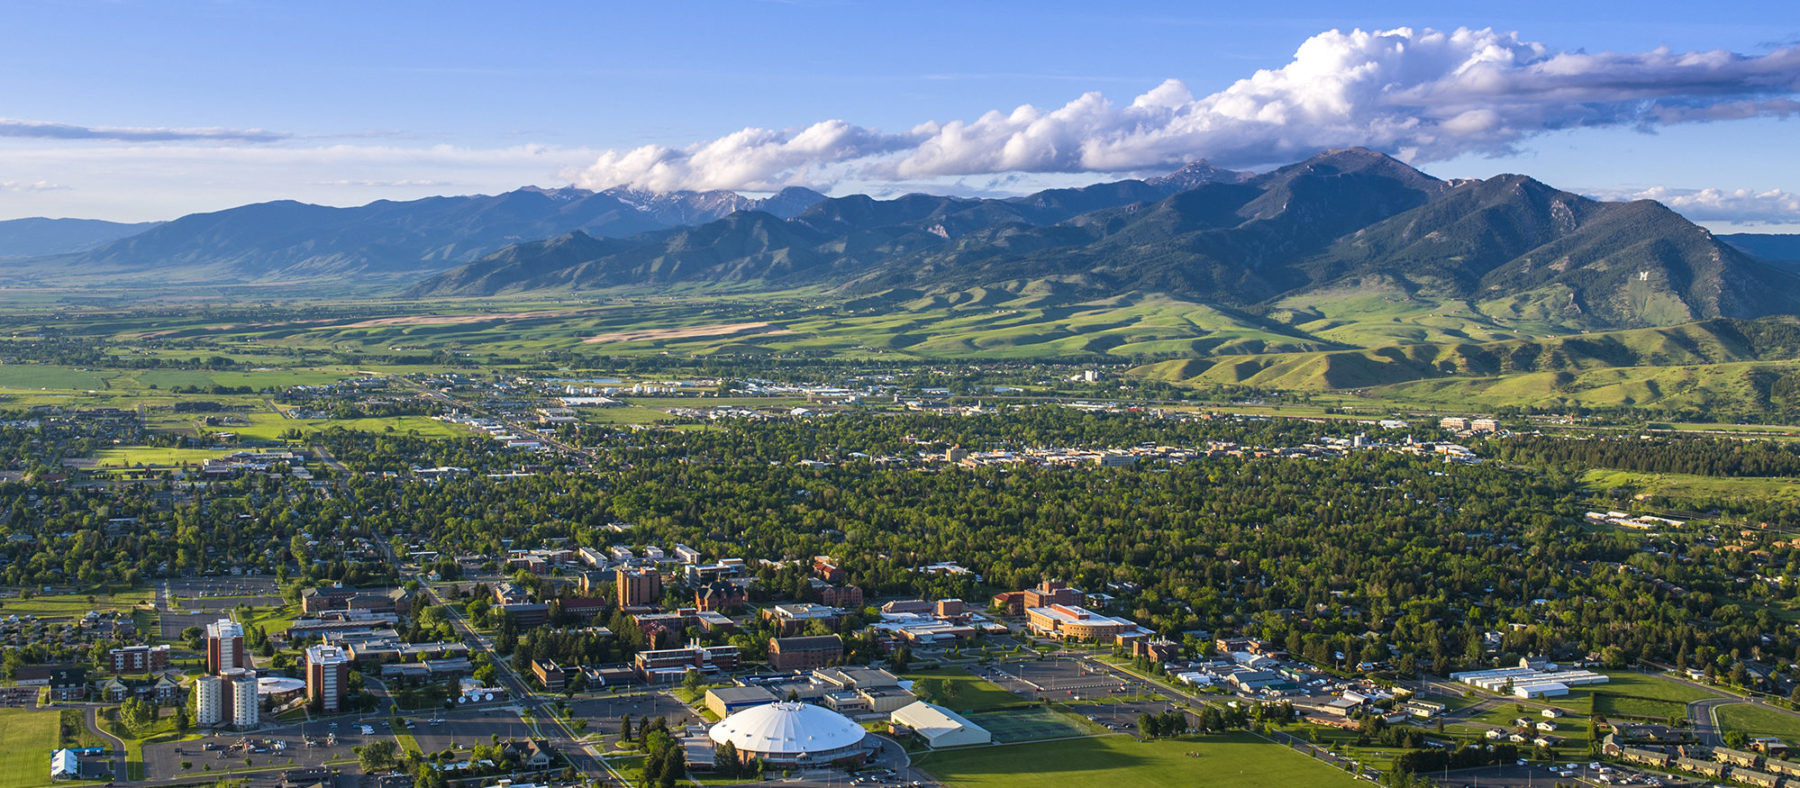
\includegraphics[width=5in,height=\textheight]{images/msu-campus.jpg}
\vspace{1cm}\\
STAT 216 Activity Coursepack}
\usepackage{etoolbox}
\makeatletter
\providecommand{\subtitle}[1]{% add subtitle to \maketitle
  \apptocmd{\@title}{\par {\large #1 \par}}{}{}
}
\makeatother
\subtitle{Fall 2020}
\author{}
\date{\vspace{-2.5em}}

\begin{document}
\maketitle

{
\setcounter{tocdepth}{0}
\tableofcontents
}
\hypertarget{preface}{%
\chapter*{Preface}\label{preface}}
\addcontentsline{toc}{chapter}{Preface}

This coursepack accompanies the textbook for STAT 216: Introduction to Statistics at Montana State University. Each of the activities in this workbook is designed to target specific learning outcomes of the course, giving you practice with important statistical concepts in a group setting with instructor guidance. Bring this workbook with you to class each week, and take notes in the workbook as you would your own notes. A well-written complete workbook will provide an optimal study guide for exams!

\hypertarget{fall-2020-calendar-of-in-class-activities}{%
\chapter*{Fall 2020 Calendar of In-Class Activities}\label{fall-2020-calendar-of-in-class-activities}}
\addcontentsline{toc}{chapter}{Fall 2020 Calendar of In-Class Activities}

Placeholder

\hypertarget{martian-alphabet}{%
\chapter{Martian Alphabet}\label{martian-alphabet}}

Placeholder

\hypertarget{learning-outcomes}{%
\section{Learning outcomes}\label{learning-outcomes}}

\hypertarget{terminology-review}{%
\section{Terminology review}\label{terminology-review}}

\hypertarget{can-you-read-martian}{%
\section{Can you read ``Martian''?}\label{can-you-read-martian}}

\hypertarget{steps-of-the-statistical-investigation-process}{%
\subsection{Steps of the statistical investigation process}\label{steps-of-the-statistical-investigation-process}}

\hypertarget{take-home-messages}{%
\section{Take home messages}\label{take-home-messages}}

\hypertarget{additional-notes}{%
\section{Additional notes}\label{additional-notes}}

\hypertarget{study-design}{%
\chapter{Study Design}\label{study-design}}

Placeholder

\hypertarget{learning-outcomes}{%
\section{Learning outcomes}\label{learning-outcomes}}

\hypertarget{terminology-review}{%
\section{Terminology review}\label{terminology-review}}

\hypertarget{types-of-sampling-bias}{%
\section{Types of sampling bias}\label{types-of-sampling-bias}}

\hypertarget{study-design-1}{%
\section{Study design}\label{study-design-1}}

\hypertarget{additional-notes}{%
\section{Additional notes}\label{additional-notes}}

\hypertarget{current-population-survey}{%
\chapter{Current Population Survey}\label{current-population-survey}}

\hypertarget{learning-outcomes}{%
\section{Learning outcomes}\label{learning-outcomes}}

\begin{itemize}
\item
  Identify and create appropriate summary statistics and plots
  given a data set or research question
\item
  Plots for a single categorical variable: bar plot
\item
  Plots for association between two categorical variables:
  segmented bar plot, mosaic plot
\item
  Recognize and simulate probabilities as long-run frequencies
\item
  Construct two-way tables to evaluate conditional probabilities
\end{itemize}

\hypertarget{terminology-review}{%
\section{Terminology review}\label{terminology-review}}

In today's activity, we will review summary measures and plots for categorical variables. Some terms covered in this activity are:

\begin{itemize}
\item
  Proportions
\item
  Bar plots
\item
  Segmented bar plots
\item
  Probability
\item
  Conditional probability
\item
  Two-way tables
\end{itemize}

To review these concepts see Sections 2.1 and 2.2 in the textbook.

\newpage

\hypertarget{current-population-survey-1985}{%
\section{``Current'' Population Survey: 1985}\label{current-population-survey-1985}}

The data set we will use for this activity is from the Current Population Survey in 1985. The CPS is a survey sponsored by the Census Bureau and the Bureau of Labor Statistics to track labor force statistics for the United States population. The following table summarizes the data:

\begin{center}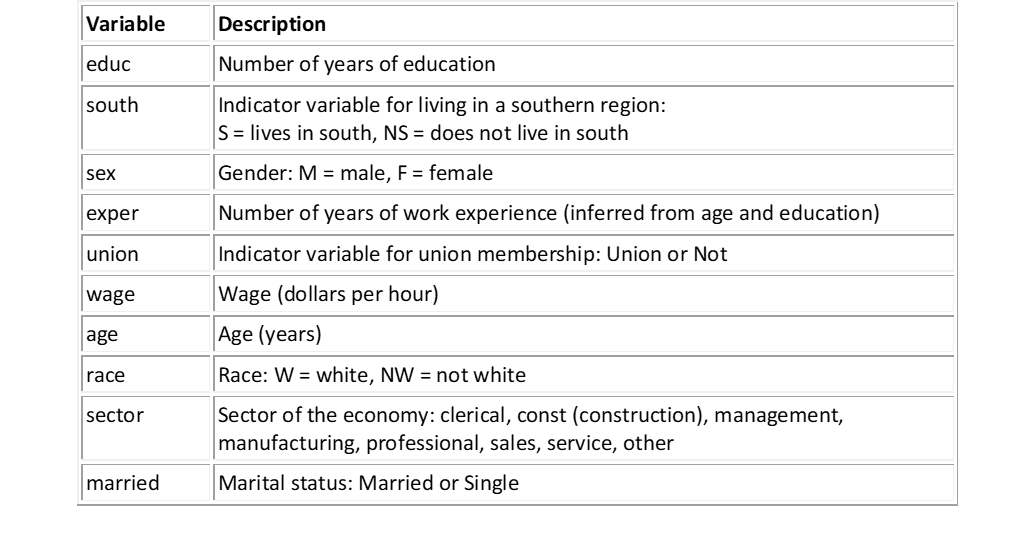
\includegraphics[width=0.7\linewidth]{images/cps} \end{center}

\hypertarget{vocabulary-review}{%
\subsection{Vocabulary review}\label{vocabulary-review}}

\begin{enumerate}
\def\labelenumi{\arabic{enumi}.}
\tightlist
\item
  What are the observational units?
\end{enumerate}

\vspace{0.2in}

\begin{enumerate}
\def\labelenumi{\arabic{enumi}.}
\setcounter{enumi}{1}
\tightlist
\item
  Which variables are categorical?
\end{enumerate}

\vspace{0.4in}

\begin{enumerate}
\def\labelenumi{\arabic{enumi}.}
\setcounter{enumi}{2}
\tightlist
\item
  What types of plots can be used to display categorical data?
\end{enumerate}

\vspace{0.5in}

An important part of understanding data is to create visual pictures of what the data represent. In this activity we will create graphical representations of categorical data.

\hypertarget{r-code}{%
\subsection{\texorpdfstring{\texttt{R} code}{R code}}\label{r-code}}

Throughout these activities, we will often include the \texttt{R} code
you would use in order to produce output or plots. These
``code chunks'' appear in gray. In the code chunk below, we
demonstrate how to read the data set into \texttt{R} using the \texttt{read.csv()} function, and tell \texttt{R} to treat the \texttt{sector} and \texttt{sex} variables as categorical variables (``factors'').

\begin{Shaded}
\begin{Highlighting}[]
\NormalTok{cps <-}\StringTok{ }\KeywordTok{read.csv}\NormalTok{(}\StringTok{"data/cps.csv"}\NormalTok{) }\CommentTok{#This will read in the dataset}
\NormalTok{cps}\OperatorTok{$}\NormalTok{sector <-}\StringTok{ }\KeywordTok{factor}\NormalTok{(cps}\OperatorTok{$}\NormalTok{sector) }\CommentTok{#When a variable is categorical, need to make it a factor}
\NormalTok{cps}\OperatorTok{$}\NormalTok{sex <-}\StringTok{ }\KeywordTok{factor}\NormalTok{(cps}\OperatorTok{$}\NormalTok{sex)}
\end{Highlighting}
\end{Shaded}

\newpage

\hypertarget{displaying-a-single-categorical-variable}{%
\subsection{Displaying a single categorical variable}\label{displaying-a-single-categorical-variable}}

If we wanted to know how many people in our data set were in each sector, we would create a bar plot of the variable sector.

\begin{Shaded}
\begin{Highlighting}[]
\KeywordTok{ggplot}\NormalTok{(}\DataTypeTok{data =}\NormalTok{ cps,   }\CommentTok{#This specifies the dataset}
       \KeywordTok{aes}\NormalTok{(}\DataTypeTok{y =}\NormalTok{ sector)) }\OperatorTok{+}\StringTok{   }\CommentTok{#This specifies the variable}
\StringTok{  }\KeywordTok{geom_bar}\NormalTok{(}\DataTypeTok{stat =} \StringTok{"count"}\NormalTok{) }\OperatorTok{+}\StringTok{  }\CommentTok{#Tell it to make a bar plot}
\StringTok{  }\KeywordTok{labs}\NormalTok{(}\DataTypeTok{title =} \StringTok{"Frequency Bar Plot of Sector"}\NormalTok{,  }\CommentTok{#Give your plot a title}
       \DataTypeTok{x =} \StringTok{"Frequency"}\NormalTok{,   }\CommentTok{#Label the x axis}
       \DataTypeTok{y =} \StringTok{"Sector"}\NormalTok{)  }\OperatorTok{+}\StringTok{ }\CommentTok{#Label the y axis}
\StringTok{  }\KeywordTok{coord_flip}\NormalTok{()  }\CommentTok{#Turn the bars so they are vertical}
\end{Highlighting}
\end{Shaded}

\begin{center}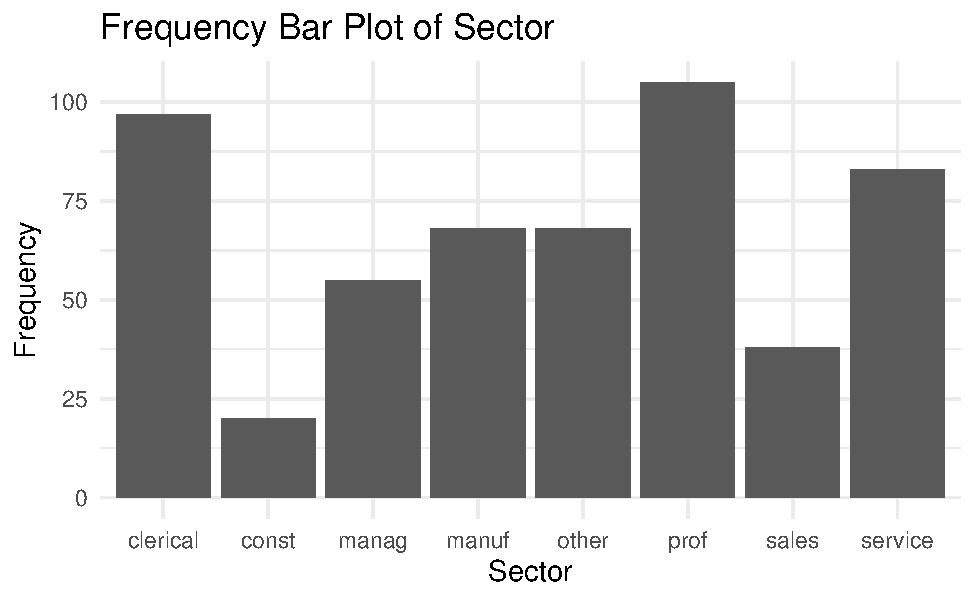
\includegraphics[width=0.5\linewidth]{03-EDA-categorical_files/figure-latex/unnamed-chunk-3-1} \end{center}

\begin{enumerate}
\def\labelenumi{\arabic{enumi}.}
\setcounter{enumi}{3}
\tightlist
\item
  Which Sector has the largest number of people in it?
\end{enumerate}

\vspace{0.3in}

We could also choose to display the data as a proportion in a relative frequency bar plot. To find the relative frequency divide the count in each sector by the sample size. These are sample proportions.

\begin{Shaded}
\begin{Highlighting}[]
\KeywordTok{ggplot}\NormalTok{(}\DataTypeTok{data =}\NormalTok{ cps,   }\CommentTok{#This specifies the dataset}
       \KeywordTok{aes}\NormalTok{(}\DataTypeTok{x =}\NormalTok{ sector)) }\OperatorTok{+}\StringTok{   }\CommentTok{#This specifies the variable}
\StringTok{  }\KeywordTok{geom_bar}\NormalTok{(}\KeywordTok{aes}\NormalTok{(}\DataTypeTok{y =}\NormalTok{ ..prop.., }\DataTypeTok{group =} \DecValTok{1}\NormalTok{)) }\OperatorTok{+}\StringTok{  }\CommentTok{#Tell it to make a bar plot with proportions}
\StringTok{  }\KeywordTok{labs}\NormalTok{(}\DataTypeTok{title =} \StringTok{"Relative Frequency Bar Plot of Sector"}\NormalTok{,  }\CommentTok{#Give your plot a title}
       \DataTypeTok{x =} \StringTok{"Sector"}\NormalTok{,   }\CommentTok{#Label the x axis}
       \DataTypeTok{y =} \StringTok{"Relative Frequency"}\NormalTok{)  }\CommentTok{#Label the y axis}
\end{Highlighting}
\end{Shaded}

\begin{center}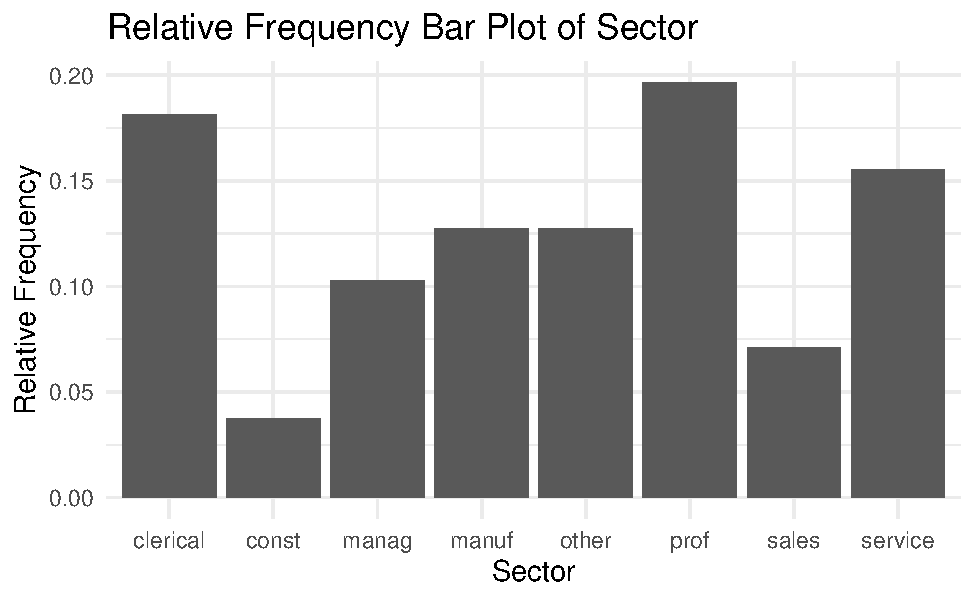
\includegraphics[width=0.5\linewidth]{03-EDA-categorical_files/figure-latex/unnamed-chunk-4-1} \end{center}

\begin{enumerate}
\def\labelenumi{\arabic{enumi}.}
\setcounter{enumi}{4}
\tightlist
\item
  Which features in the relative frequency bar plot are the same as the frequency bar plot? Which are different?
\end{enumerate}

\vspace{1in}

\hypertarget{displaying-two-categorical-variables}{%
\subsection{Displaying two categorical variables}\label{displaying-two-categorical-variables}}

To see the differences in proportion of each sector between males and females we would create a segmented bar plot of sector segmented by sex.

\begin{Shaded}
\begin{Highlighting}[]
\KeywordTok{ggplot}\NormalTok{(}\DataTypeTok{data =}\NormalTok{ cps,   }\CommentTok{#This specifies the dataset}
       \KeywordTok{aes}\NormalTok{(}\DataTypeTok{x =}\NormalTok{ sector, }\DataTypeTok{fill =}\NormalTok{ sex)) }\OperatorTok{+}\StringTok{   }\CommentTok{#This specifies the variables}
\StringTok{  }\KeywordTok{geom_bar}\NormalTok{(}\DataTypeTok{stat =} \StringTok{"count"}\NormalTok{, }\DataTypeTok{position =} \StringTok{"fill"}\NormalTok{) }\OperatorTok{+}\StringTok{  }\CommentTok{#Tell it to make a stacked bar plot}
\StringTok{  }\KeywordTok{labs}\NormalTok{(}\DataTypeTok{title =} \StringTok{"Segmented Bar Plot of Sector by Sex"}\NormalTok{,  }\CommentTok{#Make sure to title your plot }
       \DataTypeTok{x =} \StringTok{"Sector"}\NormalTok{,   }\CommentTok{#Label the x axis}
       \DataTypeTok{y =} \StringTok{""}\NormalTok{) }\OperatorTok{+}\StringTok{  }\CommentTok{#Remove y axis label}
\StringTok{    }\KeywordTok{scale_fill_grey}\NormalTok{()  }\CommentTok{#Make figure black and white}
\end{Highlighting}
\end{Shaded}

\begin{center}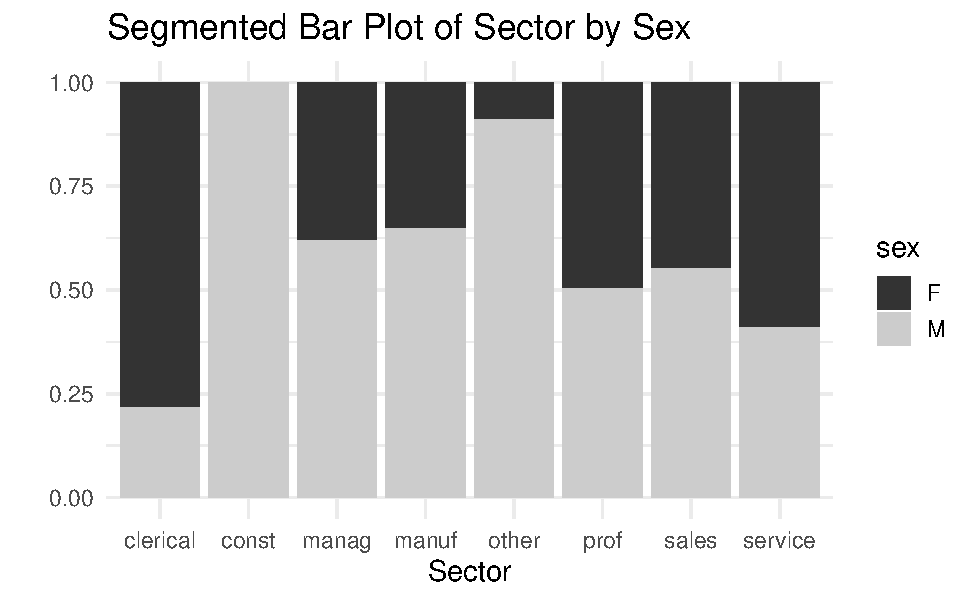
\includegraphics[width=0.6\linewidth]{03-EDA-categorical_files/figure-latex/unnamed-chunk-5-1} \end{center}

\begin{enumerate}
\def\labelenumi{\arabic{enumi}.}
\setcounter{enumi}{5}
\tightlist
\item
  Using the segmented bar plot, which sector has about the same proportion of males and females?
\end{enumerate}

\vspace{0.5in}

\begin{enumerate}
\def\labelenumi{\arabic{enumi}.}
\setcounter{enumi}{6}
\tightlist
\item
  Which sector has the highest proportion of females?
\end{enumerate}

\vspace{0.5in}

\begin{enumerate}
\def\labelenumi{\arabic{enumi}.}
\setcounter{enumi}{7}
\tightlist
\item
  Which variable is the explanatory variable? Which is the response variable?
\end{enumerate}

\newpage

\hypertarget{probability}{%
\section{Probability}\label{probability}}

\begin{enumerate}
\def\labelenumi{\arabic{enumi}.}
\setcounter{enumi}{8}
\tightlist
\item
  A study was reported in which ninth grade Minnesota teens were asked whether they had gambled at least once a week in the past year. The sample consisted of 49.1\% boys. The proportion of boys who had gambled at least once per week during the past year was 0.229, while among non-boys this proportion was only 0.045.\\
  Let B = the event the person is a boy, and C = the event the person is a weekly gambler.
  \vspace{0.1in}
\end{enumerate}

\begin{enumerate}
\def\labelenumi{\alph{enumi}.}
\item
  Draw a segmented bar plot of sex segmented by gambling.
  \vspace{2in}
\item
  Identify what each numerical value represents in probability notation.
  \vspace{.1in}
\end{enumerate}

~~~~~~~~~~~~~~~~0.491 = \vspace{.2in}\\
\hspace*{0.333em}\hspace*{0.333em}\hspace*{0.333em}\hspace*{0.333em}\hspace*{0.333em}\hspace*{0.333em}\hspace*{0.333em}\hspace*{0.333em}\hspace*{0.333em}\hspace*{0.333em}\hspace*{0.333em}\hspace*{0.333em}\hspace*{0.333em}\hspace*{0.333em}\hspace*{0.333em}\hspace*{0.333em}0.229 =

\vspace{.2in}

~~~~~~~~~~~~~~~~0.045 =

\vspace{.2in}

\begin{enumerate}
\def\labelenumi{\alph{enumi}.}
\setcounter{enumi}{2}
\tightlist
\item
  Create a two-way hypothetical table to represent the situation. Recall that in a two-way table, the explanatory variable should be your column headers (similar to the x-axis in a segmented bar graph!) while the response variable becomes the row headers.
\end{enumerate}

\begin{longtable}[]{@{}llll@{}}
\toprule
\hspace{1in} & \hspace{1in} & \hspace{1in} & Total\tabularnewline
\midrule
\endhead
\hspace{1in} & & &\tabularnewline
\hspace{1in} & & &\tabularnewline
\hspace{1in} & & &\tabularnewline
Total & & & 100,000\tabularnewline
\bottomrule
\end{longtable}

\begin{enumerate}
\def\labelenumi{\alph{enumi}.}
\setcounter{enumi}{3}
\item
  Find \(P(\mbox{B and C})\). What does this probability represent in the context of the problem?
  \vspace{1in}
\item
  Find the probability that a selected non-gambler is a non-boy. What is the notation used for this probability?
\end{enumerate}

\newpage

\begin{enumerate}
\def\labelenumi{\arabic{enumi}.}
\setcounter{enumi}{9}
\tightlist
\item
  In a computer store, 30\% of the computers in stock are laptops and 70\% are desktops. Five percent of the laptops are on sale, while 10\% of the desktops are on sale. Let L = the event the computer is a laptop, and S = the event the computer is on sale.
  \vspace{0.1in}
\end{enumerate}

\begin{enumerate}
\def\labelenumi{\alph{enumi}.}
\tightlist
\item
  Identify what each numerical value represents in probability notation.
  \vspace{.1in}
\end{enumerate}

~~~~~~~~~~~~~~~~0.30 = \vspace{.2in}\\
\hspace*{0.333em}\hspace*{0.333em}\hspace*{0.333em}\hspace*{0.333em}\hspace*{0.333em}\hspace*{0.333em}\hspace*{0.333em}\hspace*{0.333em}\hspace*{0.333em}\hspace*{0.333em}\hspace*{0.333em}\hspace*{0.333em}\hspace*{0.333em}\hspace*{0.333em}\hspace*{0.333em}\hspace*{0.333em}0.70 =

\vspace{.2in}

~~~~~~~~~~~~~~~~0.05 =

\vspace{.2in}

~~~~~~~~~~~~~~~~0.10 =

\vspace{.2in}

\begin{enumerate}
\def\labelenumi{\alph{enumi}.}
\setcounter{enumi}{1}
\tightlist
\item
  Create a two-way table to represent the situation.
\end{enumerate}

\begin{longtable}[]{@{}llll@{}}
\toprule
\hspace{1in} & \hspace{1in} & \hspace{1in} & Total\tabularnewline
\midrule
\endhead
\hspace{1in} & & &\tabularnewline
\hspace{1in} & & &\tabularnewline
\hspace{1in} & & &\tabularnewline
Total & & & 100,000\tabularnewline
\bottomrule
\end{longtable}

\begin{enumerate}
\def\labelenumi{\alph{enumi}.}
\setcounter{enumi}{2}
\item
  Calculate the probability that a randomly selected computer will be a desktop, given that the computer is on sale. What is the notation used for this probability?
  \vspace{1in}
\item
  Find \(P(S | L^C)\). What does this probability represent in context of the problem?
  \vspace{1in}
\end{enumerate}

\hypertarget{additional-notes}{%
\section{Additional notes}\label{additional-notes}}

Use this space to summarize your thoughts and take additional notes on today's activity.

\hypertarget{imdb-movie-reviews}{%
\chapter{IMDb Movie Reviews}\label{imdb-movie-reviews}}

Placeholder

\hypertarget{learning-objectives}{%
\section{Learning objectives}\label{learning-objectives}}

\hypertarget{terminology-review}{%
\section{Terminology review}\label{terminology-review}}

\hypertarget{movies-released-in-2016}{%
\section{Movies released in 2016}\label{movies-released-in-2016}}

\hypertarget{vocabulary-review}{%
\section{Vocabulary review}\label{vocabulary-review}}

\hypertarget{summarizing-a-single-quantitative-variable}{%
\section{Summarizing a single quantitative variable}\label{summarizing-a-single-quantitative-variable}}

\hypertarget{displaying-a-single-quantitative-variable}{%
\section{Displaying a single quantitative variable}\label{displaying-a-single-quantitative-variable}}

\hypertarget{displaying-a-single-categorical-and-single-quantitative-variable}{%
\section{Displaying a single categorical and single quantitative variable}\label{displaying-a-single-categorical-and-single-quantitative-variable}}

\hypertarget{additional-notes}{%
\section{Additional notes}\label{additional-notes}}

\hypertarget{movie-profits}{%
\chapter{Movie Profits}\label{movie-profits}}

Placeholder

\hypertarget{learning-objectives}{%
\section{Learning objectives}\label{learning-objectives}}

\hypertarget{terminology-review}{%
\section{Terminology review}\label{terminology-review}}

\hypertarget{movies-released-in-2016}{%
\section{Movies released in 2016}\label{movies-released-in-2016}}

\hypertarget{vocabulary-review}{%
\subsection{Vocabulary review}\label{vocabulary-review}}

\hypertarget{correlation}{%
\subsection{Correlation}\label{correlation}}

\hypertarget{slope}{%
\subsection{Slope}\label{slope}}

\hypertarget{residuals}{%
\subsection{Residuals}\label{residuals}}

\hypertarget{coefficient-of-determination-r-squared}{%
\subsection{Coefficient of determination (R-squared)}\label{coefficient-of-determination-r-squared}}

\hypertarget{multivariate-plots}{%
\subsection{Multivariate plots}\label{multivariate-plots}}

\hypertarget{additional-notes}{%
\section{Additional notes}\label{additional-notes}}

\hypertarget{handedness-of-male-boxers}{%
\chapter{Handedness of Male Boxers}\label{handedness-of-male-boxers}}

Placeholder

\hypertarget{learning-objectives}{%
\section{Learning objectives}\label{learning-objectives}}

\hypertarget{terminology-review}{%
\section{Terminology review}\label{terminology-review}}

\hypertarget{steps-of-the-statistical-investigation-process}{%
\section{Steps of the statistical investigation process}\label{steps-of-the-statistical-investigation-process}}

\hypertarget{handedness-of-male-boxers-1}{%
\section{Handedness of male boxers}\label{handedness-of-male-boxers-1}}

\hypertarget{summary-statistics-review}{%
\subsection{Summary statistics review}\label{summary-statistics-review}}

\hypertarget{ask-a-research-question}{%
\subsection{Ask a research question}\label{ask-a-research-question}}

\hypertarget{design-a-study-and-collect-data}{%
\subsection{Design a study and collect data}\label{design-a-study-and-collect-data}}

\hypertarget{summarize-and-visualize-the-data}{%
\subsection{Summarize and visualize the data}\label{summarize-and-visualize-the-data}}

\hypertarget{use-statistical-analysis-methods-to-draw-inferences-from-the-data}{%
\subsection{Use statistical analysis methods to draw inferences from the data}\label{use-statistical-analysis-methods-to-draw-inferences-from-the-data}}

\hypertarget{communicate-the-results-and-answer-the-research-question}{%
\subsection{Communicate the results and answer the research question}\label{communicate-the-results-and-answer-the-research-question}}

\hypertarget{revisit-and-look-forward}{%
\subsection{Revisit and look forward}\label{revisit-and-look-forward}}

\hypertarget{additional-notes}{%
\section{Additional notes}\label{additional-notes}}

\hypertarget{winter-sports-helmet-use-and-head-injuries}{%
\chapter{Winter Sports Helmet Use and Head Injuries}\label{winter-sports-helmet-use-and-head-injuries}}

Placeholder

\hypertarget{learning-objectives}{%
\section{Learning objectives}\label{learning-objectives}}

\hypertarget{terminology-review}{%
\section{Terminology review}\label{terminology-review}}

\hypertarget{helmet-use-and-head-injuries}{%
\section{Helmet Use and Head Injuries}\label{helmet-use-and-head-injuries}}

\hypertarget{vocabulary-review}{%
\subsection{Vocabulary review}\label{vocabulary-review}}

\hypertarget{ask-a-research-question}{%
\subsection{Ask a research question}\label{ask-a-research-question}}

\hypertarget{summarize-and-visualize-the-data}{%
\subsection{Summarize and visualize the data}\label{summarize-and-visualize-the-data}}

\hypertarget{use-statistical-analysis-methods-to-draw-inferences-from-the-data}{%
\subsection{Use statistical analysis methods to draw inferences from the data}\label{use-statistical-analysis-methods-to-draw-inferences-from-the-data}}

\hypertarget{types-of-errors}{%
\subsection{Types of errors}\label{types-of-errors}}

\hypertarget{additional-notes}{%
\section{Additional notes}\label{additional-notes}}

\hypertarget{covid-19-and-air-pollution}{%
\chapter{COVID-19 and Air Pollution}\label{covid-19-and-air-pollution}}

Placeholder

\hypertarget{learning-outcomes}{%
\section{Learning outcomes}\label{learning-outcomes}}

\hypertarget{terminology-review}{%
\section{Terminology review}\label{terminology-review}}

\hypertarget{covid-19-and-air-pollution-1}{%
\section{COVID-19 and air pollution}\label{covid-19-and-air-pollution-1}}

\hypertarget{vocabulary-review}{%
\subsection{Vocabulary review}\label{vocabulary-review}}

\hypertarget{ask-a-research-question}{%
\subsection{Ask a research question}\label{ask-a-research-question}}

\hypertarget{summarize-and-visualize-the-data}{%
\subsection{Summarize and visualize the data}\label{summarize-and-visualize-the-data}}

\hypertarget{use-statistical-inferential-methods-to-draw-inferences-from-the-data}{%
\subsection{Use statistical inferential methods to draw inferences from the data}\label{use-statistical-inferential-methods-to-draw-inferences-from-the-data}}

\hypertarget{communicate-the-results-and-answer-the-research-question.}{%
\subsection{Communicate the results and answer the research question.}\label{communicate-the-results-and-answer-the-research-question.}}

\hypertarget{revisit-and-look-forward}{%
\subsection{Revisit and look forward}\label{revisit-and-look-forward}}

\hypertarget{additional-notes}{%
\section{Additional notes}\label{additional-notes}}

\hypertarget{weather-patterns-and-record-snowfall}{%
\chapter{Weather Patterns and Record Snowfall}\label{weather-patterns-and-record-snowfall}}

Placeholder

\hypertarget{learning-objectives}{%
\section{Learning objectives}\label{learning-objectives}}

\hypertarget{terminology-review}{%
\section{Terminology review}\label{terminology-review}}

\hypertarget{weather-patterns-and-record-snowfall-1}{%
\section{Weather Patterns and Record snowfall}\label{weather-patterns-and-record-snowfall-1}}

\hypertarget{quantitative-variables-review}{%
\subsection{Quantitative variables review}\label{quantitative-variables-review}}

\hypertarget{ask-a-research-question.}{%
\subsection{Ask a research question.}\label{ask-a-research-question.}}

\hypertarget{summarize-and-visualize-the-data}{%
\subsection{Summarize and visualize the data}\label{summarize-and-visualize-the-data}}

\hypertarget{use-statistical-inferential-methods-to-draw-inferences-from-the-data}{%
\subsection{Use statistical inferential methods to draw inferences from the data}\label{use-statistical-inferential-methods-to-draw-inferences-from-the-data}}

\hypertarget{communicate-the-results-and-answer-the-research-question}{%
\subsection{Communicate the results and answer the research question}\label{communicate-the-results-and-answer-the-research-question}}

\hypertarget{revisit-and-look-rorward}{%
\subsection{Revisit and look rorward}\label{revisit-and-look-rorward}}

\hypertarget{additional-notes}{%
\section{Additional notes}\label{additional-notes}}

\hypertarget{hand-dexterity}{%
\chapter{Hand Dexterity}\label{hand-dexterity}}

Placeholder

\hypertarget{learning-outcomes}{%
\section{Learning outcomes}\label{learning-outcomes}}

\hypertarget{terminology-review}{%
\section{Terminology review}\label{terminology-review}}

\hypertarget{hand-dexterity-1}{%
\section{Hand dexterity}\label{hand-dexterity-1}}

\hypertarget{vocabulary-review}{%
\subsection{Vocabulary review}\label{vocabulary-review}}

\hypertarget{conditions-for-the-least-squares-line}{%
\subsection{Conditions for the least squares line}\label{conditions-for-the-least-squares-line}}

\hypertarget{ask-a-research-question}{%
\subsection{Ask a research question}\label{ask-a-research-question}}

\hypertarget{summarize-and-visualize-the-data}{%
\subsection{Summarize and visualize the data}\label{summarize-and-visualize-the-data}}

\hypertarget{use-statistical-inferential-methods-to-draw-inferences-from-the-data}{%
\subsection{Use statistical inferential methods to draw inferences from the data}\label{use-statistical-inferential-methods-to-draw-inferences-from-the-data}}

\hypertarget{communicate-the-results-and-answer-the-research-question}{%
\subsection{Communicate the results and answer the research question}\label{communicate-the-results-and-answer-the-research-question}}

\hypertarget{revisit-and-look-forward}{%
\subsection{Revisit and look forward}\label{revisit-and-look-forward}}

\hypertarget{additional-notes}{%
\section{Additional notes}\label{additional-notes}}

\end{document}
